\documentclass[12pt]{article}
\usepackage[a4paper, margin=1in]{geometry}
\usepackage{graphicx}
\usepackage{dirtree}
\usepackage{amsmath}
\usepackage{hyperref}
\usepackage{listings}
\usepackage{color}
\usepackage{enumitem}
\usepackage{titlesec}

% Define subsubsubsection
\titleclass{\subsubsubsection}{straight}[\subsubsection]
\newcounter{subsubsubsection}[subsubsection]
\renewcommand\thesubsubsubsection{\thesubsubsection.\arabic{subsubsubsection}}
\titleformat{\subsubsubsection}
  {\normalfont\normalsize\bfseries}{\thesubsubsubsection}{1em}{}
\titlespacing*{\subsubsubsection}{0pt}{1ex plus .2ex}{1ex plus .2ex}

% Set up code listing style
\definecolor{codegray}{gray}{0.95}
\lstset{
    backgroundcolor=\color{codegray},
    basicstyle=\ttfamily\small,
    frame=single,
    breaklines=true,
    captionpos=b
}

\titleformat{\section}{\large\bfseries}{\thesection}{1em}{}

\title{\textbf{Angry Birds Game Project Report}}
\author{Sayan Mandal \\ \small CS-104}
\date{Spring 2024-2025}

\begin{document}

\maketitle
\tableofcontents
\newpage

\section{Introduction}
The main objective of making this game is to extend the single-player version of the original Angry Birds game to a turn-by-turn based two-player game where each player aims to destroy the opponents fortress by launching projectile from his slingshot.

\section{Modules}
The external modules used are:
\begin{itemize}
    \item \textbf{pygame} – Used for game rendering, event handling, and graphics management.
    \item \textbf{math} – Provides mathematical functions such as trigonometry, used in projectile motion calculations.
    \item \textbf{random} – Used to generate random positions or parameters for objects.
    \item \textbf{numpy} - Used to create arrays of objects and work on them
\end{itemize}

\section{Directory Structure}
The structure of the project directory is as follows:
\dirtree{%
    .1 \hspace{1.5pt}..
    .2 Scripts.
    .3 Game.py.
    .3 MainMenu.py.
    .3 birds.py.
    .3 blocks.py.
    .3 utils.py.
    .2 Media.
    .3 Fonts.
    .3 Sprites.
    .2 Data.
    .3 GameHistory.csv.
    .2 main.py.
}
\begin{itemize}
    \item \textbf{Scripts} – Various scripts that manages various parts of the game
    \item \textbf{Media} - Contains sprites and fonts used in the game
    \item \textbf{Data} – Contains player scores of the last 10 games played
    \item \textbf{main.py} – Main game loop
\end{itemize}

\section{Running Instructions}
\subsection{Installation}
Python must be installed on the device prior to this. Then the pygame module must be installed using the following command:
\begin{verbatim}
pip install pygame
\end{verbatim}

\subsection{Execution}
To run the program, open the terminal in the directory containing "main.py" and then use one of the following commands whichever is suitable.
\begin{verbatim}
python main.py
python3 main.py
\end{verbatim}

\subsection{Game Navigation and Gameplay}
\subsubsection{Main Menu Screen}
The Main Menu screen is first shown as the game begins. Here, the user can choose to:
\begin{itemize}
    \item Play
    \item History(See the scores of past 10 matches)
    \item Quit
\end{itemize}
\subsubsection{Game Settings}
After selecting to play the game, the Game Settings screen opens where the name of the players can be entered. The following game settings can also be changed:
\begin{itemize}
     \item \textbf{Fortress dimensions} - Change the dimensions of the fortress (rows X columns).
    \item \textbf{Number of birds in queue} - To specify the maximum number of birds each player gets at a time. Note that once all the birds get used up new set of birds are randomly provided.
    \item \textbf{Include block gravity} – Option to include gravity for blocks which acts at the end of turn of each player
    \item \textbf{Include predicted projectile} – Option to display the predicted projectile upon dragging the bird on slingshot
\end{itemize}

\subsubsection{Loading Screen}
After confirming the game settings, the loading screen appears. With a countdown of 3 seconds the match starts.

\subsubsection{Match}
The match begins with player1(left) who has to aim his projectile at player2's(right) fortress. The turn ends after the projectile comes to a halt, or falls underneath the screen or spends a considerable amount of time outside the side boundaries of the screen. Then begins the turn of player2 who has to aim his projectile at player1's fortress and the game continues. \\
\subsubsubsection{Controls}
\begin{itemize}
    \item Click and drag to stretch the slingshot.
    \item Release the mouse button to launch the projectile.
\end{itemize}\\

\subsubsubsection{Blocks}
The following table describes the type of blocks in the game:
\begin{table}[h!]
\centering
\label{tab:Blocks}
\begin{tabular}{@{}|l|l|c|@{}}
\toprule
\hline
\textbf{Block Type} & \textbf{Weaker to} & \textbf{Number of Images} \\
\midrule
\hline
Wood & Red,Chuck & 4 \\
\hline
Stone & Red,Bomb & 4 \\
\hline
Ice & Red,Blue & 4 \\
\hline
\bottomrule
\end{tabular}
\caption{Types of Blocks}
\end{table}\\
Blocks are randomly generated to create the fortress. Each player's fortress is the mirror image of the other to maintain fairness.\\

\subsubsubsection{Birds}
The following table describes the type of projectiles/birds in the game:
\begin{table}[h!]
\centering
\label{tab:Birds}
\begin{tabular}{@{}|l|l|@{}}
\toprule
\hline
\textbf{Bird Type} & \textbf{Strength}  \\
\midrule
\hline
Red & Wood,Stone,Ice \\
\hline
Chuck & Wood  \\
\hline
Bomb & Stone \\
\hline
Blue & Ice \\
\hline
\bottomrule
\end{tabular}
\caption{Types of Birds}
\end{table}\\
Birds in the queue are randomly generated for each players separately. Birds in queue closer to the center of the screen are picked up first.\\
Images of the Birds are taken from internet sources.\\

\subsubsubsection{Block Damage}
The damage that the projectile does to the blocks it hits is proportional to its normal velocity to the block. If the block is destroyed then the projectile losses some amount of its velocity, whereas it bounces with a velocity having a reduced normal component.\\
\subsubsubsection{Scoring system}
Scores at each turn are assigned to the player based on the following equation:
\begin{equation}
    score = \frac{damage\cdot health}{1000} + 3\cdot B
\end{equation}
where, damage = Health of the block reduced by the projectile,\\
       health = Health of the block before hitting it (maximum 100)\\
       \begin{equation*}
       B = 
       \begin{cases}
        1 & \text{if projectile's first hit block is its strength and the projectile is not Red Bird} \\
        0 & \text{otherwise}
       \end{cases}
       \end{equation*}
This is done to ensure reward for precise aim. Upon successfully destroying the opponent's fortress completely, the player is rewarded with an extra 20 points.\\

\subsubsubsection{Winning Condition}
The game ends when one of the player's fortress is completely destroyed with an exception (as player1 destroys player2's fortress player2 is given a last chance before game ends as player1 starts the game first). This maintains fairness in the game.\\ 
When game ends the player with greater score wins. The scores of the players are then stored in history which can be viewed from the Main Menu. The players can then choose to either play again or return to the Main Menu.\\

\subsubsection{Game History}
On clicking "HISTORY" in Main Menu the names of players along with their scores are loaded for last 10 matches.\\

\section{Basic and Advanced Features}
\subsection{Basic Features}
\begin{itemize}
    \item Slingshot mechanic using mouse drag.
    \item Basic projectile physics with parabolic motion.
    \item Collision detection with targets or environment.
\end{itemize}

\subsection{Advanced Features}
\begin{itemize}
    \item Block Gravity that applies after each turn
    \item Predicted projectile on dragging the bird on slingshot
    \item Breaking the block at different extent based on its health
    \item Storing scores of players for last 10 matches
    \item Scoring system based on precision and accuracy of the destruction caused by the projectile
    \item Self-made background, slingshot, block and platform images
\end{itemize}\\

\section{Screenshots}
The following are some the screenshots from the game:
\begin{figure}[h!]
    \centering
    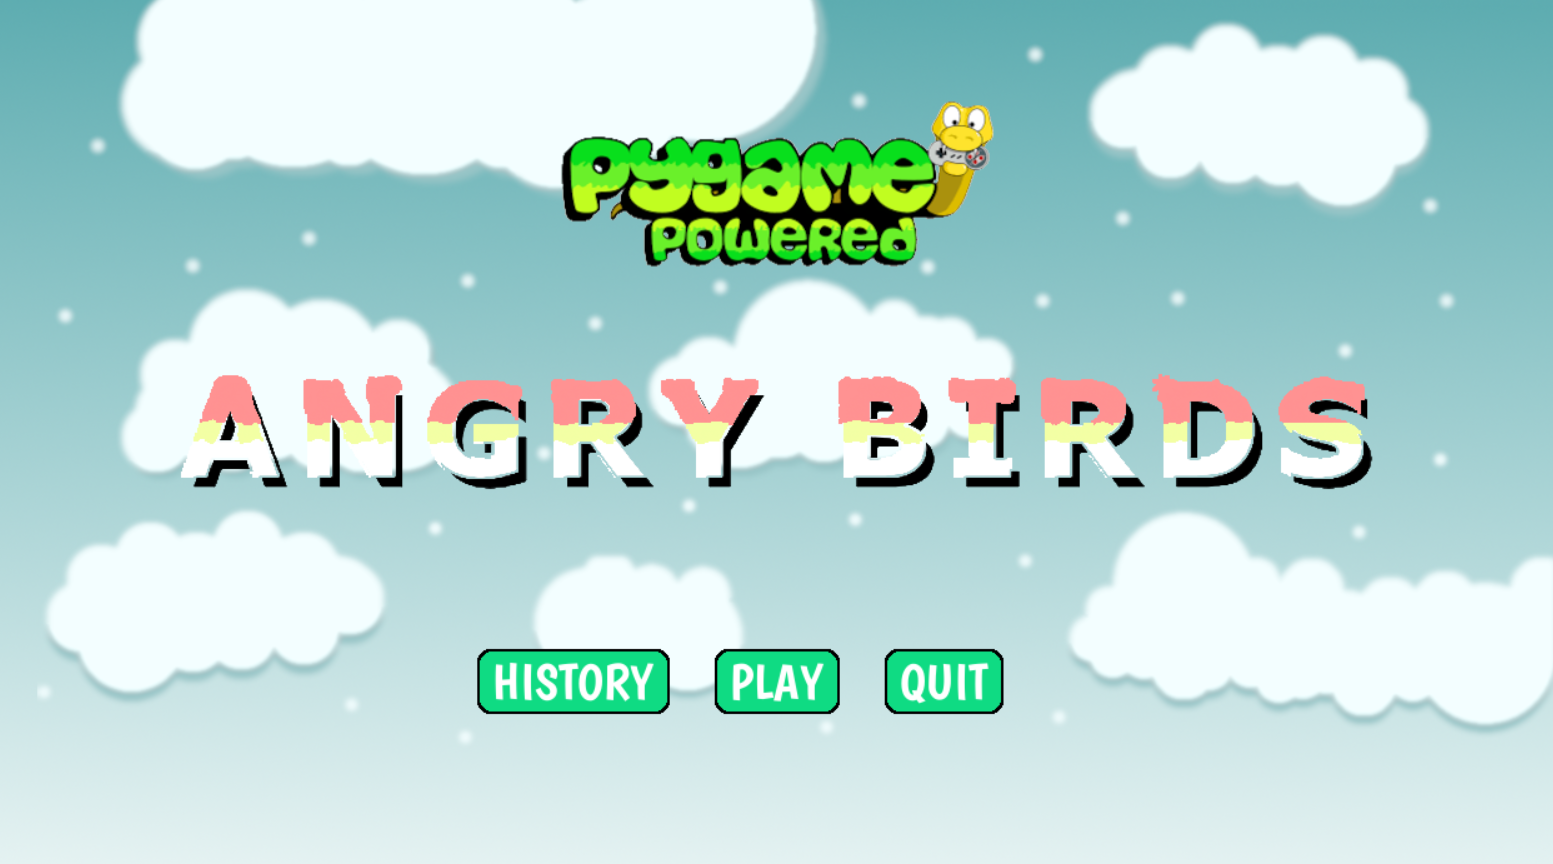
\includegraphics[width=0.7\textwidth]{ScreenShots/TitleScreen.png}
    \caption{Title Screen}
\end{figure}

\begin{figure}[h!]
    \centering
    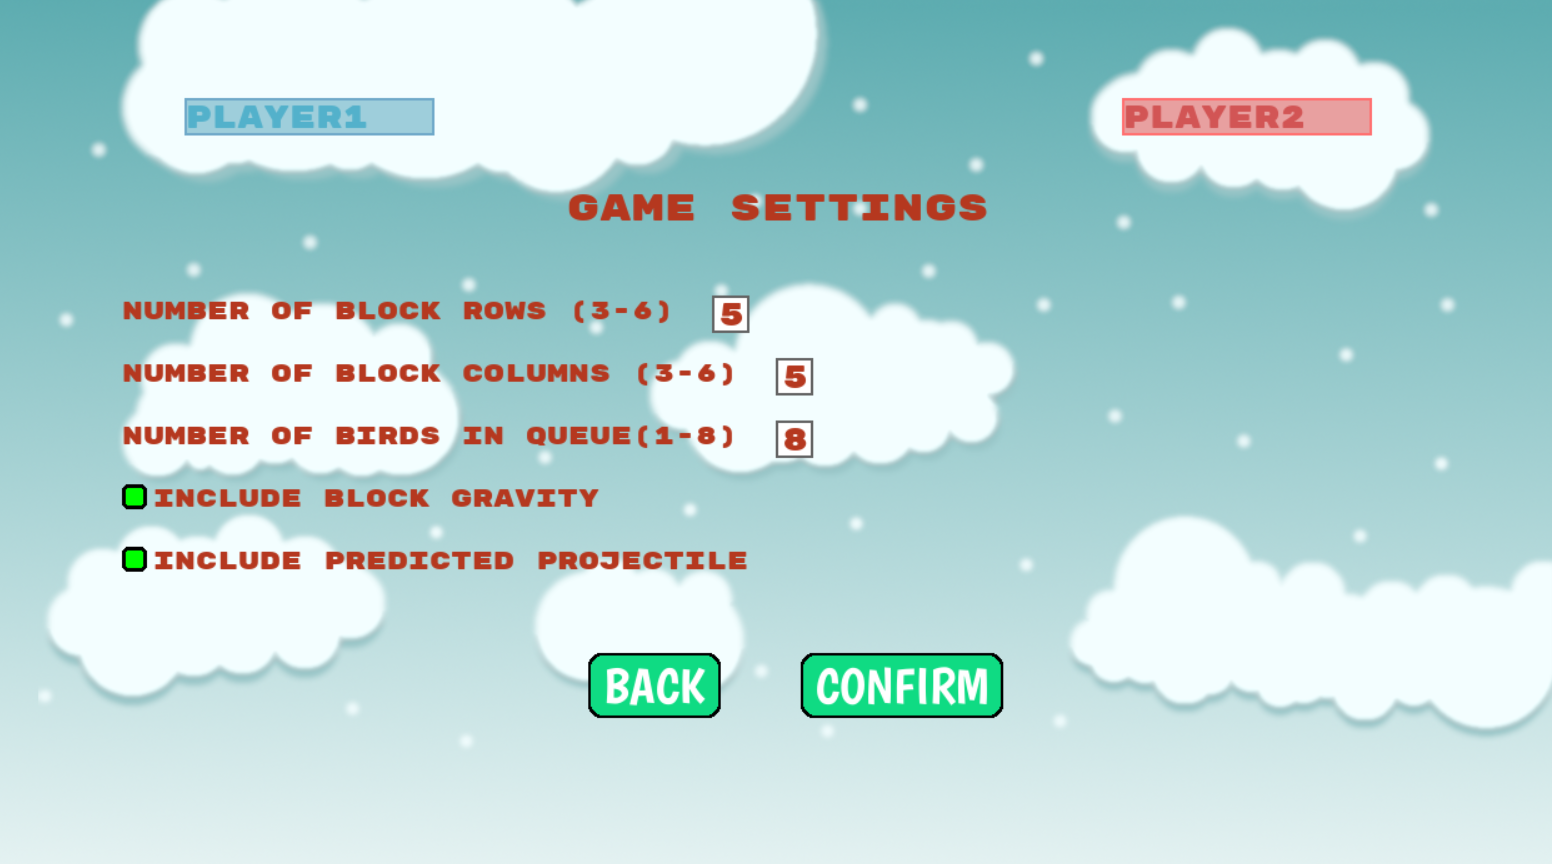
\includegraphics[width=0.7\textwidth]{ScreenShots/GameSettings.png}
    \caption{Game Settings Screen}
\end{figure}

\begin{figure}[h!]
    \centering
    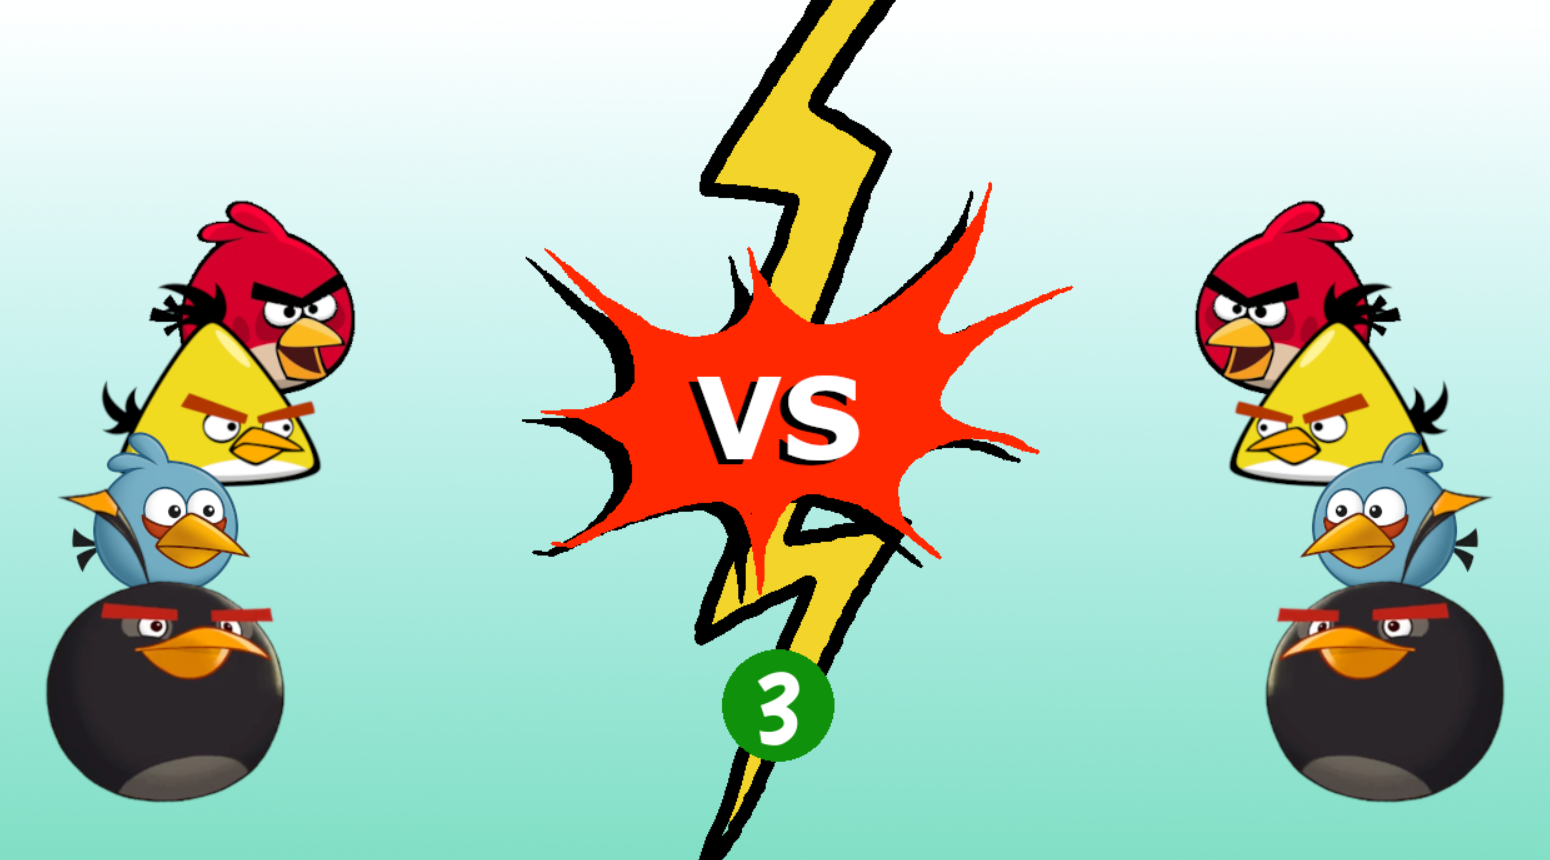
\includegraphics[width=0.7\textwidth]{ScreenShots/LoadingScreen.png}
    \caption{Loading Screen}
\end{figure}

\begin{figure}[h!]
    \centering
    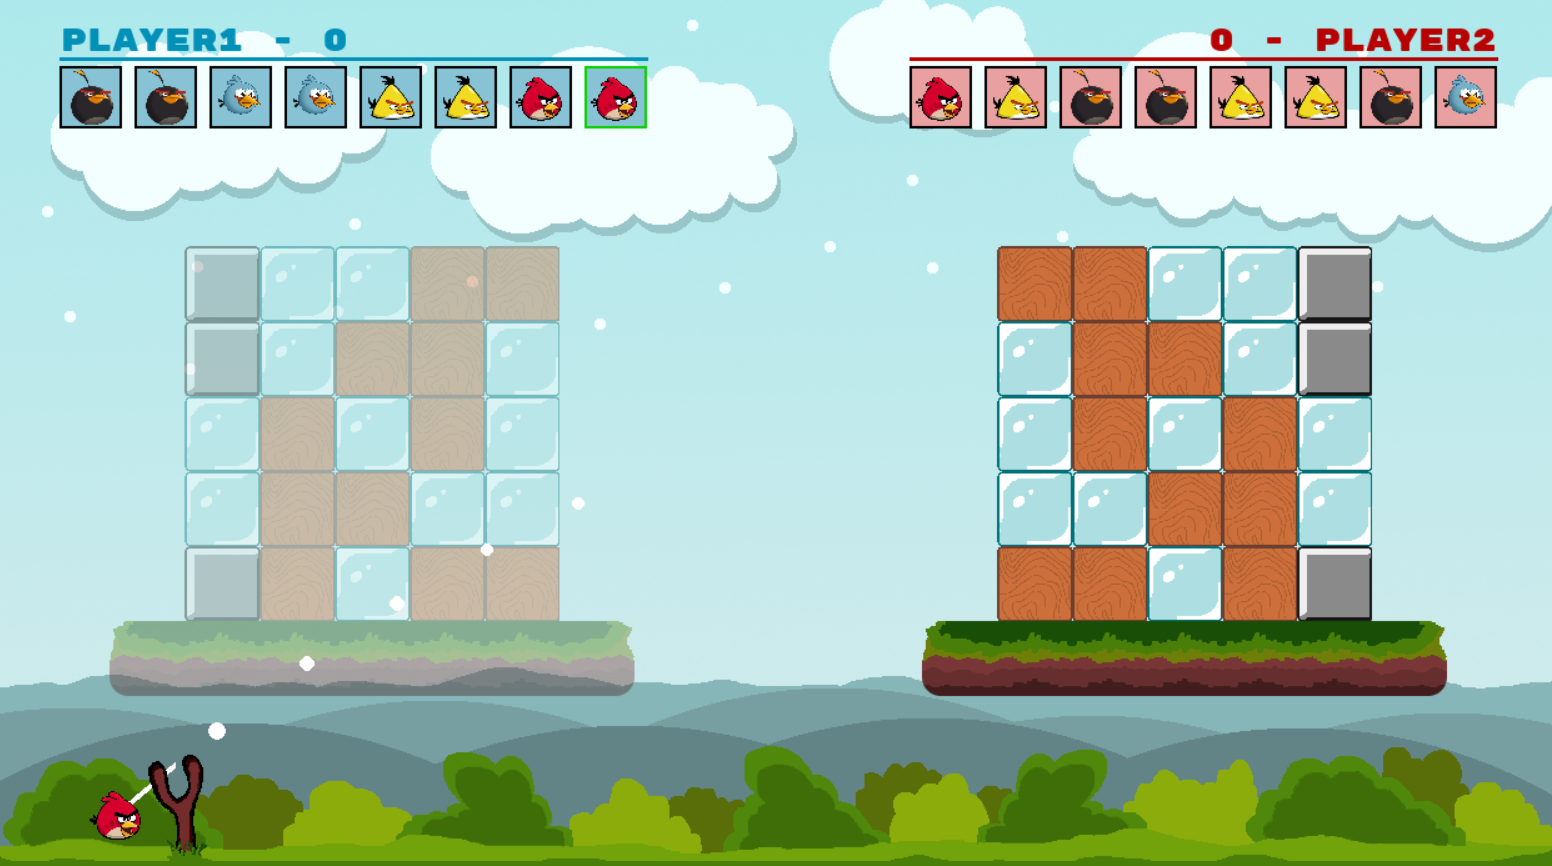
\includegraphics[width=0.7\textwidth]{ScreenShots/GameStarts.png}
    \caption{Game Starts}
\end{figure}

\begin{figure}[h!]
    \centering
    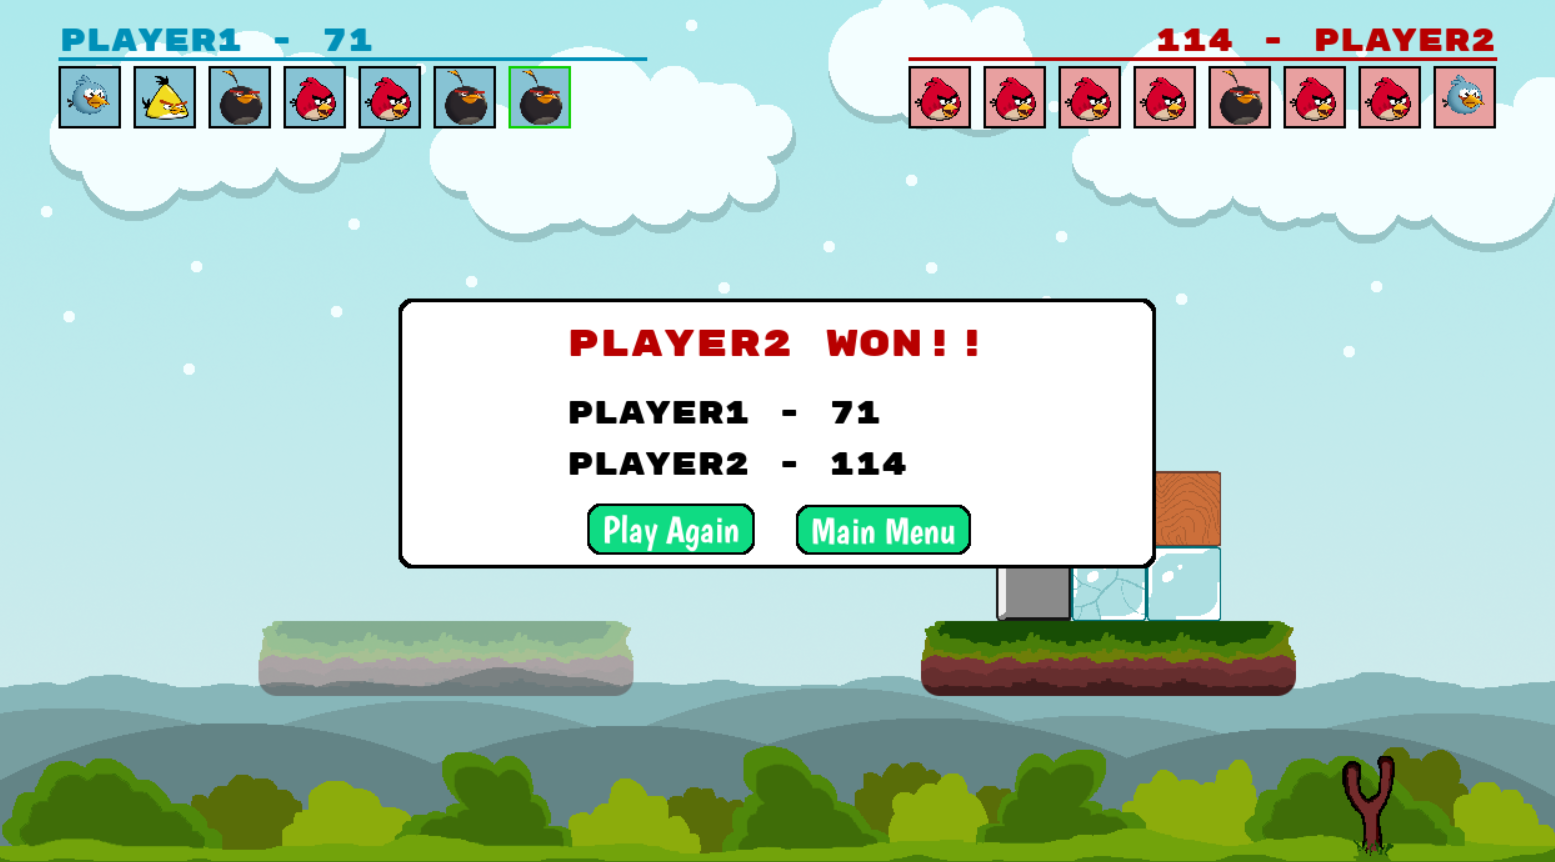
\includegraphics[width=0.7\textwidth]{ScreenShots/GameEnds.png}
    \caption{Game Ends}
\end{figure}

\begin{figure}[h!]
    \centering
    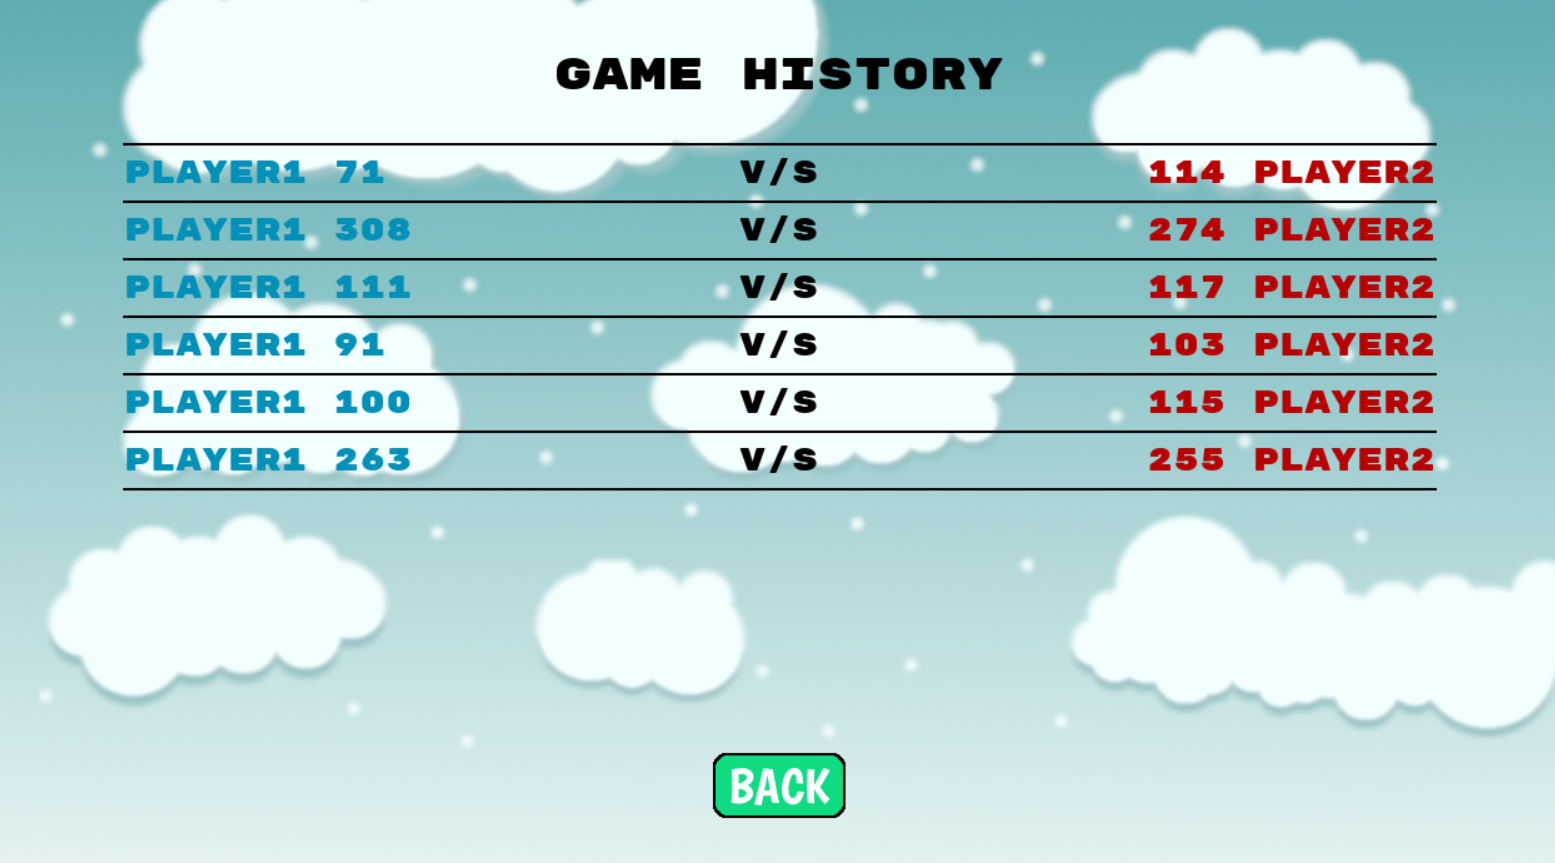
\includegraphics[width=0.7\textwidth]{ScreenShots/GameHistory.png}
    \caption{Game History}
\end{figure}

\newpage

\section{Project Journey}
\subsection{Key Learnings}
\begin{itemize}
    \item Understanding of basic physics and how to simulate motion.
    \item Hands-on experience with event-driven programming using Pygame.
\end{itemize}

\subsection{Challenges and Solutions}
\begin{itemize}
    \item \textbf{Physics inaccuracies:} Fine-tuned projectile formulas and implemented frame-independent movement.
    \item \textbf{Collision glitches:} Adjusted hitbox size and used self-made collision detection utilities.
\end{itemize}

\section{Bibliography}
\begin{itemize}
    \item Pygame Documentation: \url{https://www.pygame.org/docs/}
    \item Physics of Projectiles: \url{https://ocw.mit.edu/courses/8-01sc-classical-mechanics-fall-2016/796b8c575392e081439a7d4f10f820be_MIT8_01F16_chapter5.2.pdf}
    \item Bird Images: Internet source
\end{itemize}

\end{document}
